% Generated by ICLR_Q4.py from experiment_logs_Q4 -- Drone4D_x0set: Total runtime [s]
% Shaded band = min/max over seeds; line = median over seeds.
% Picture width is exactly \linewidth. Requires \usepackage{pgfplots}.
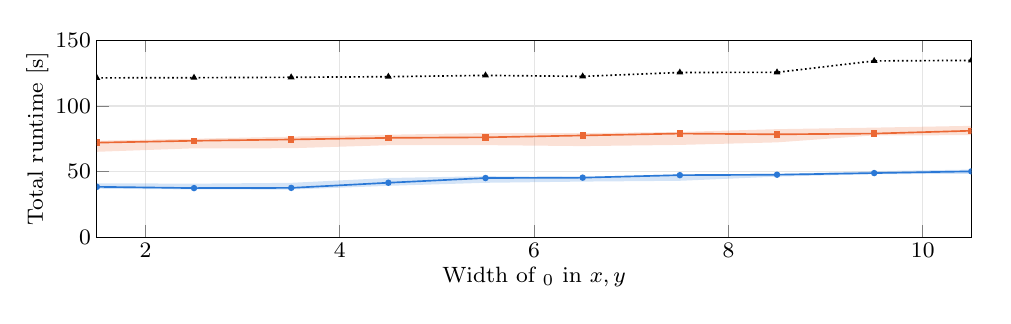
\begin{tikzpicture}[baseline=(current axis.south)]
\definecolor{q4ppo}{RGB}{42,120,214}
\definecolor{q4sac}{RGB}{235,104,52}
\definecolor{q4dense}{RGB}{0,0,0}
\begin{axis}[
    scale only axis, width=\linewidth-25pt-4pt, height=2.5cm,
    xlabel={Width of $\X_0$ in $x,y$},
    ylabel={Total runtime [s]}, ylabel style={align=center},
    xmin=1.5, xmax=10.5, xtick={2,4,6,8,10},
    ymin=0, ymax=150, ytick={0,50,100,150},
    grid=major, grid style={gray!20}, clip marker paths=true,
    label style={font=\footnotesize}, tick label style={font=\footnotesize, inner sep=2pt},
    xlabel shift=-2pt, ylabel shift=-3pt,  % labels close to the tick labels
]
% PPO: 5 seeds per X0 span
\addplot[draw=none, fill=q4ppo, fill opacity=0.2, forget plot] coordinates {(1.5,36.943) (2.5,36.4193) (3.5,36.2862) (4.5,39.1303) (5.5,41.4421) (6.5,42.3687) (7.5,42.9795) (8.5,46.1563) (9.5,48.0422) (10.5,48.3178) (10.5,51.5103) (9.5,50.3494) (8.5,48.2333) (7.5,47.9066) (6.5,45.9376) (5.5,46.4973) (4.5,45.0999) (3.5,41.4188) (2.5,40.7996) (1.5,41.106)} -- cycle;
\addplot[q4ppo, semithick, mark=*, mark size=0.85pt] coordinates {(1.5,38.3778) (2.5,37.4156) (3.5,37.5686) (4.5,41.492) (5.5,45.081) (6.5,45.3668) (7.5,47.2769) (8.5,47.6097) (9.5,48.8671) (10.5,50.1497)};
% SAC: 5 seeds per X0 span
\addplot[draw=none, fill=q4sac, fill opacity=0.2, forget plot] coordinates {(1.5,65.0665) (2.5,67.7267) (3.5,67.7845) (4.5,70.1071) (5.5,70.1528) (6.5,69.4144) (7.5,70.3135) (8.5,72.2586) (9.5,77.5874) (10.5,77.7245) (10.5,84.8415) (9.5,83.4859) (8.5,82.3169) (7.5,80.1923) (6.5,79.3013) (5.5,79.3646) (4.5,78.0795) (3.5,76.6222) (2.5,75.035) (1.5,73.5015)} -- cycle;
\addplot[q4sac, semithick, mark=square*, mark size=0.85pt] coordinates {(1.5,72.0344) (2.5,73.461) (3.5,74.4472) (4.5,75.6932) (5.5,76.0961) (6.5,77.5104) (7.5,78.9612) (8.5,78.3844) (9.5,78.9615) (10.5,81.1042)};
% Dense (single deterministic run per X0 span)
\addplot[q4dense, semithick, mark=triangle*, mark size=0.85pt, densely dotted, mark options={solid}] coordinates {(1.5,121.39) (2.5,121.538) (3.5,121.833) (4.5,122.307) (5.5,123.286) (6.5,122.546) (7.5,125.505) (8.5,125.631) (9.5,134.307) (10.5,134.718)};
\end{axis}
% Fix the bounding box to exactly \linewidth wide: the axis box plus the label margins
\path (current axis.south west |- current bounding box.south) ++(-25pt,0) coordinate (q4sw)
      (current axis.north east |- current bounding box.north) ++(4pt,0) coordinate (q4ne);
\pgfresetboundingbox
\useasboundingbox (q4sw) rectangle (q4ne);
\end{tikzpicture}%
